% ============================================================
%  AIP Final Project – 15-Slide Beamer Presentation
%  Topic: FreeTTA (Online EM) vs TDA (Cache-Based) with CLIP ViT-B/16
%  Compile: pdflatex slides.tex  (run from presentation/ directory)
% ============================================================
\documentclass[aspectratio=169,11pt]{beamer}

\usetheme{Madrid}
\usecolortheme{default}

\definecolor{primary}{RGB}{31,119,180}
\definecolor{accent}{RGB}{214,39,40}
\definecolor{darkgray}{RGB}{60,60,60}
\definecolor{lightbg}{RGB}{245,248,252}
\definecolor{green2}{RGB}{44,162,95}
\definecolor{gold}{RGB}{220,170,30}

\setbeamercolor{palette primary}{bg=primary, fg=white}
\setbeamercolor{palette secondary}{bg=primary!80, fg=white}
\setbeamercolor{palette tertiary}{bg=primary!60, fg=white}
\setbeamercolor{frametitle}{bg=primary, fg=white}
\setbeamercolor{title}{fg=white}
\setbeamercolor{structure}{fg=primary}
\setbeamercolor{block title}{bg=primary!15, fg=primary}
\setbeamercolor{block body}{bg=lightbg}
\setbeamercolor{alertblock title}{bg=accent!20, fg=accent!80!black}
\setbeamercolor{alertblock body}{bg=accent!5}
\setbeamercolor{exampleblock title}{bg=green2!20, fg=green2!70!black}
\setbeamercolor{exampleblock body}{bg=green2!5}

\usepackage{amsmath,amssymb,bm}
\usepackage{booktabs}
\usepackage{graphicx}
\usepackage{xcolor}
\usepackage{array}
\usepackage{colortbl}
\usepackage{fontawesome5}

\graphicspath{{../outputs/deep_analysis/}}

\setbeamersize{text margin left=4mm,text margin right=4mm}
\setbeamertemplate{navigation symbols}{}
\setbeamertemplate{footline}{%
  \leavevmode
  \hbox{%
    \begin{beamercolorbox}[wd=.33\paperwidth,ht=2.25ex,dp=1ex,center]{author in head/foot}%
      \usebeamerfont{author in head/foot}\insertshortauthor
    \end{beamercolorbox}%
    \begin{beamercolorbox}[wd=.34\paperwidth,ht=2.25ex,dp=1ex,center]{title in head/foot}%
      \usebeamerfont{title in head/foot}\insertshorttitle
    \end{beamercolorbox}%
    \begin{beamercolorbox}[wd=.33\paperwidth,ht=2.25ex,dp=1ex,right]{date in head/foot}%
      \usebeamerfont{date in head/foot}\insertframenumber{} / \inserttotalframenumber\hspace{2pt}
    \end{beamercolorbox}}%
}

\newcommand{\highlight}[1]{\textcolor{accent}{\textbf{#1}}}
\newcommand{\blue}[1]{\textcolor{primary}{\textbf{#1}}}
\newcommand{\green}[1]{\textcolor{green2}{\textbf{#1}}}
\newcommand{\tick}{\textcolor{green2}{\faCheck}}
\newcommand{\cross}{\textcolor{accent}{\faTimes}}
\newcommand{\mub}{\boldsymbol{\mu}}

\title[FreeTTA vs TDA]{Test-Time Adaptation with CLIP:\\
\large FreeTTA (Online EM) vs.\ TDA (Cache-Based)}
\author[Herry Saraswat]{Herry Saraswat}
\institute{[University Name]}
\date{April 2026}

\begin{document}

%% ─────────────────────────────────────────────────────────────────────────────
%% SLIDE 1 – TITLE
%% ─────────────────────────────────────────────────────────────────────────────
{
\setbeamertemplate{footline}{}
\setbeamercolor{background canvas}{bg=primary}
\begin{frame}[plain]
\vfill
\begin{center}
  {\color{white}\LARGE\textbf{Test-Time Adaptation with CLIP}}\\[10pt]
  {\color{white!85}\large FreeTTA (Online EM) vs.\ TDA (Cache-Based)}\\[6pt]
  {\color{accent!50!white}\rule{0.55\textwidth}{0.8pt}}\\[18pt]
  {\color{white}\large Herry Saraswat}\\[6pt]
  {\color{white!80}\normalsize [University Name]}\\[6pt]
  {\color{white!70}\small April 2026}
\end{center}
\vfill
\end{frame}
}

%% ─────────────────────────────────────────────────────────────────────────────
%% SLIDE 2 – MOTIVATION
%% ─────────────────────────────────────────────────────────────────────────────
\begin{frame}{Motivation: Why Test-Time Adaptation?}
\begin{columns}[T]
\column{0.49\textwidth}
  \begin{block}{The Core Problem}
    \begin{itemize}\footnotesize\setlength{\itemsep}{2pt}
      \item CLIP trained on web data, deployed on specialist domains\\
            (satellite images, textures, pet breeds)
      \item At test time: \textbf{no labels, no gradients, frozen backbone}
      \item CLIP entropy $\approx\log C$ on all 5 benchmarks — maximally uncertain
      \item Goal: adapt predictions using only the test stream
    \end{itemize}
  \end{block}
  \vspace{3pt}
  \begin{exampleblock}{\footnotesize Shared Constraint}
    \footnotesize Both methods operate on \textbf{frozen CLIP features} only.\\
    No retraining. No labels. Pure inference-time adaptation.
  \end{exampleblock}
\column{0.49\textwidth}
  \begin{block}{Two Competing Strategies}
    \begin{itemize}\footnotesize\setlength{\itemsep}{2pt}
      \item \textbf{TDA}: memory-based — stores confident exemplars in a per-class cache; retrieves them at query time
      \item \textbf{FreeTTA}: statistics-based — maintains running class-mean estimates via online EM; no per-sample storage
    \end{itemize}
  \end{block}
  \vspace{3pt}
  \begin{alertblock}{\footnotesize Research Question}
    \footnotesize When and why does each method win?\\
    We run \textbf{13+ analyses} across 5 datasets and 26,114 samples to find out.
  \end{alertblock}
\end{columns}
\end{frame}

%% ─────────────────────────────────────────────────────────────────────────────
%% SLIDE 3 – TDA ARCHITECTURE
%% ─────────────────────────────────────────────────────────────────────────────
\begin{frame}{Baseline: TDA (Test-Time Dynamic Adapter)}
\begin{columns}[T]
\column{0.50\textwidth}
  \begin{block}{Algorithm per Test Sample}
    \footnotesize
    \textbf{1.} Compute CLIP logits\;
    $\mathbf{l}_{\rm clip} = \tau\cdot\hat{\mathbf{x}}^\top\mathbf{W}$\\[3pt]
    \textbf{2.} Route by normalised entropy $H_{\rm norm} = H/\log C$:
    \begin{itemize}\footnotesize\setlength{\itemsep}{1pt}
      \item $H_{\rm norm} < 0.2$\;: add to \blue{positive cache}
      \item $0.2 < H_{\rm norm} < 0.5$\;: also add to \highlight{negative cache}
    \end{itemize}
    \textbf{3.} Cache affinity (vectorised einsum):
    \[\text{aff}_{c,s} = \hat{\mathbf{x}}^\top \hat{\mathbf{f}}_{c,s}\]
    \textbf{4.} Fused logits:
    \[\mathbf{l}_{\rm TDA} = \mathbf{l}_{\rm clip} + \alpha\mathbf{l}^+ - \alpha'\mathbf{l}^-\]
    \textbf{5.} Cache eviction: remove highest-entropy slot if full
  \end{block}
\column{0.48\textwidth}
  \begin{exampleblock}{Design Properties}
    \begin{itemize}\footnotesize\setlength{\itemsep}{2pt}
      \item Positive cache: $C \times K$ slots (e.g.\ $100{\times}3{=}300$ for Caltech)
      \item Eviction policy: keep lowest-entropy (most confident) exemplars
      \item Memory: $O(C \cdot K \cdot D)$;\quad Time: $O(C \cdot K)$ per sample
      \item Cache fills within \textbf{first 20\%} of stream; then eviction-only
    \end{itemize}
  \end{exampleblock}
  \begin{alertblock}{\footnotesize Known Weakness}
    \footnotesize Negative-cache gate $[0.2,0.5]$ structurally fires \textbf{0\%} when CLIP entropy $\equiv\log C$ (maximally uniform). Fixed capacity: learning rate $\to 0$ as cache saturates.
  \end{alertblock}
\end{columns}
\end{frame}

%% ─────────────────────────────────────────────────────────────────────────────
%% SLIDE 4 – FREETTA ARCHITECTURE
%% ─────────────────────────────────────────────────────────────────────────────
\begin{frame}{Extension: FreeTTA (Online EM Adaptation)}
\begin{columns}[T]
\column{0.50\textwidth}
  \begin{block}{EM Algorithm per Test Sample}
    \footnotesize
    \textbf{E-step} — predict using adapted means:
    \[\hat{y} = \arg\max_c\;[\mathbf{l}_{\rm clip} + \alpha(\hat{\mathbf{x}}^\top\mub_c)]\cdot\tau\]
    \textbf{Soft entropy gate} (always $>0$):
    \[\alpha_t = \exp(-\beta\cdot H_{\rm norm})\;\in(0,1]\]
    \textbf{M-step} — update class means:
    \[\mub_c \leftarrow \frac{N_c\,\mub_c + \alpha_t p_c\,\hat{\mathbf{x}}}{N_c + \alpha_t p_c},\quad N_c \leftarrow N_c + \alpha_t p_c\]
    Init: $\mub_c^{(0)} = \hat{\mathbf{t}}_c$ (CLIP text embeddings)
  \end{block}
\column{0.48\textwidth}
  \begin{exampleblock}{Design Properties}
    \begin{itemize}\footnotesize\setlength{\itemsep}{2pt}
      \item \textbf{No capacity limit} — every sample refines all class means
      \item Memory: $O(C{\cdot}D)$\;—\;5--15$\times$ less than TDA
      \item Inference time: identical to CLIP (no cache lookup)
      \item Convergence: $\mub_c(t)\to\bar{\mathbf{x}}_c$ as $N\to\infty$
    \end{itemize}
  \end{exampleblock}
  \begin{alertblock}{\footnotesize Key Advantage}
    \footnotesize Gain grows monotonically with stream length. Even small $\alpha_t$ (e.g.\ $0.05$ on Caltech) accumulates over thousands of samples. No saturation.
  \end{alertblock}
\end{columns}
\end{frame}

%% ─────────────────────────────────────────────────────────────────────────────
%% SLIDE 5 – EXPERIMENTAL SETUP
%% ─────────────────────────────────────────────────────────────────────────────
\begin{frame}{Experimental Setup}
\begin{columns}[T]
\column{0.46\textwidth}
  \begin{block}{Datasets}
    \scriptsize
    \begin{tabular}{lrrl}
      \toprule
      Dataset & $N$ & $C$ & Domain shift\\
      \midrule
      Caltech-101  & 2,465  & 100  & Low\\
      DTD          & 1,880  &  47  & Medium\\
      EuroSAT      & 8,100  &  10  & High (satellite)\\
      Oxford Pets  & 3,669  &  37  & Low (fine-grained)\\
      ImageNetV2   & 10,000 & 1000 & Low\\
      \midrule
      \textbf{Total} & \textbf{26,114} & & \\
      \bottomrule
    \end{tabular}
  \end{block}
  \vspace{3pt}
  \begin{block}{\footnotesize Per-Sample Data}
    \scriptsize
    CLIP/TDA/FreeTTA logits, entropy, confidence, EM weights, cache states, predictions — for all 26,114 samples across all 5 datasets.
  \end{block}
\column{0.52\textwidth}
  \begin{exampleblock}{Analysis Pipeline — 13 Sections}
    \begin{itemize}\scriptsize\setlength{\itemsep}{1pt}
      \item[\faChartBar] \textbf{Results}: accuracy, BFP, change rate (S1)
      \item[\faChartLine] \textbf{Adaptation dynamics}: rolling acc, break-even (S3)
      \item[\faSearch] \textbf{Scaling}: controlled SPC sweep 5\%--100\% (S9)
      \item[\faQuestion] \textbf{Uncertainty}: entropy bucket analysis (S4)
      \item[\faDatabase] \textbf{Cache pressure}: fill rate \& eviction study (S7)
      \item[\faProjectDiagram] \textbf{Distribution modeling}: centroid drift, EM (S5)
      \item[\faRuler] \textbf{GAS geometry}: centroid vs 1-NN analysis (S11, new)
      \item[\faCog] \textbf{Architecture}: LR decay, gate, logit direction (S15, new)
      \item[\faFlask] \textbf{Experiments}: neg-cache sweep, majority vote (new)
    \end{itemize}
  \end{exampleblock}
\end{columns}
\end{frame}

%% ─────────────────────────────────────────────────────────────────────────────
%% SLIDE 6 – RESULTS: ACCURACY COMPARISON
%% ─────────────────────────────────────────────────────────────────────────────
\begin{frame}{Results: Accuracy Comparison}
\begin{columns}[T]
\column{0.42\textwidth}
  \begin{block}{Reproduced Accuracy (\%)}
    \scriptsize
    \begin{tabular}{lrrl}
      \toprule
      Dataset & TDA & FreeTTA & $\Delta$ (FT$-$TDA)\\
      \midrule
      Caltech  & 93.59 & \textbf{93.63} & $+0.04$\\
      DTD      & 45.16 & \textbf{46.54} & $+1.38$\\
      EuroSAT  & 53.33 & \textbf{59.35} & $+6.01$\\
      Pets     & \textbf{88.69} & 88.63 & $-0.05$\\
      ImageNet & \textbf{62.72} & 62.72 & $0.00$\\
      \midrule
      Mean gain & $+1.16$\% & $\mathbf{+2.64}$\% & \\
      \bottomrule
    \end{tabular}
  \end{block}
  \vspace{3pt}
  \begin{block}{\footnotesize Beneficial Flip Precision}
    \scriptsize Of all changed predictions, fraction beneficial:\\[2pt]
    \begin{tabular}{lcc}
      \toprule
      Dataset & TDA & FreeTTA\\
      \midrule
      EuroSAT & 60.7\% & \textbf{77.1\%}\\
      DTD     & 62.6\% & \textbf{68.1\%}\\
      Pets    & \textbf{67.7\%} & 62.2\%\\
      \bottomrule
    \end{tabular}
  \end{block}
\column{0.56\textwidth}
  \centering
  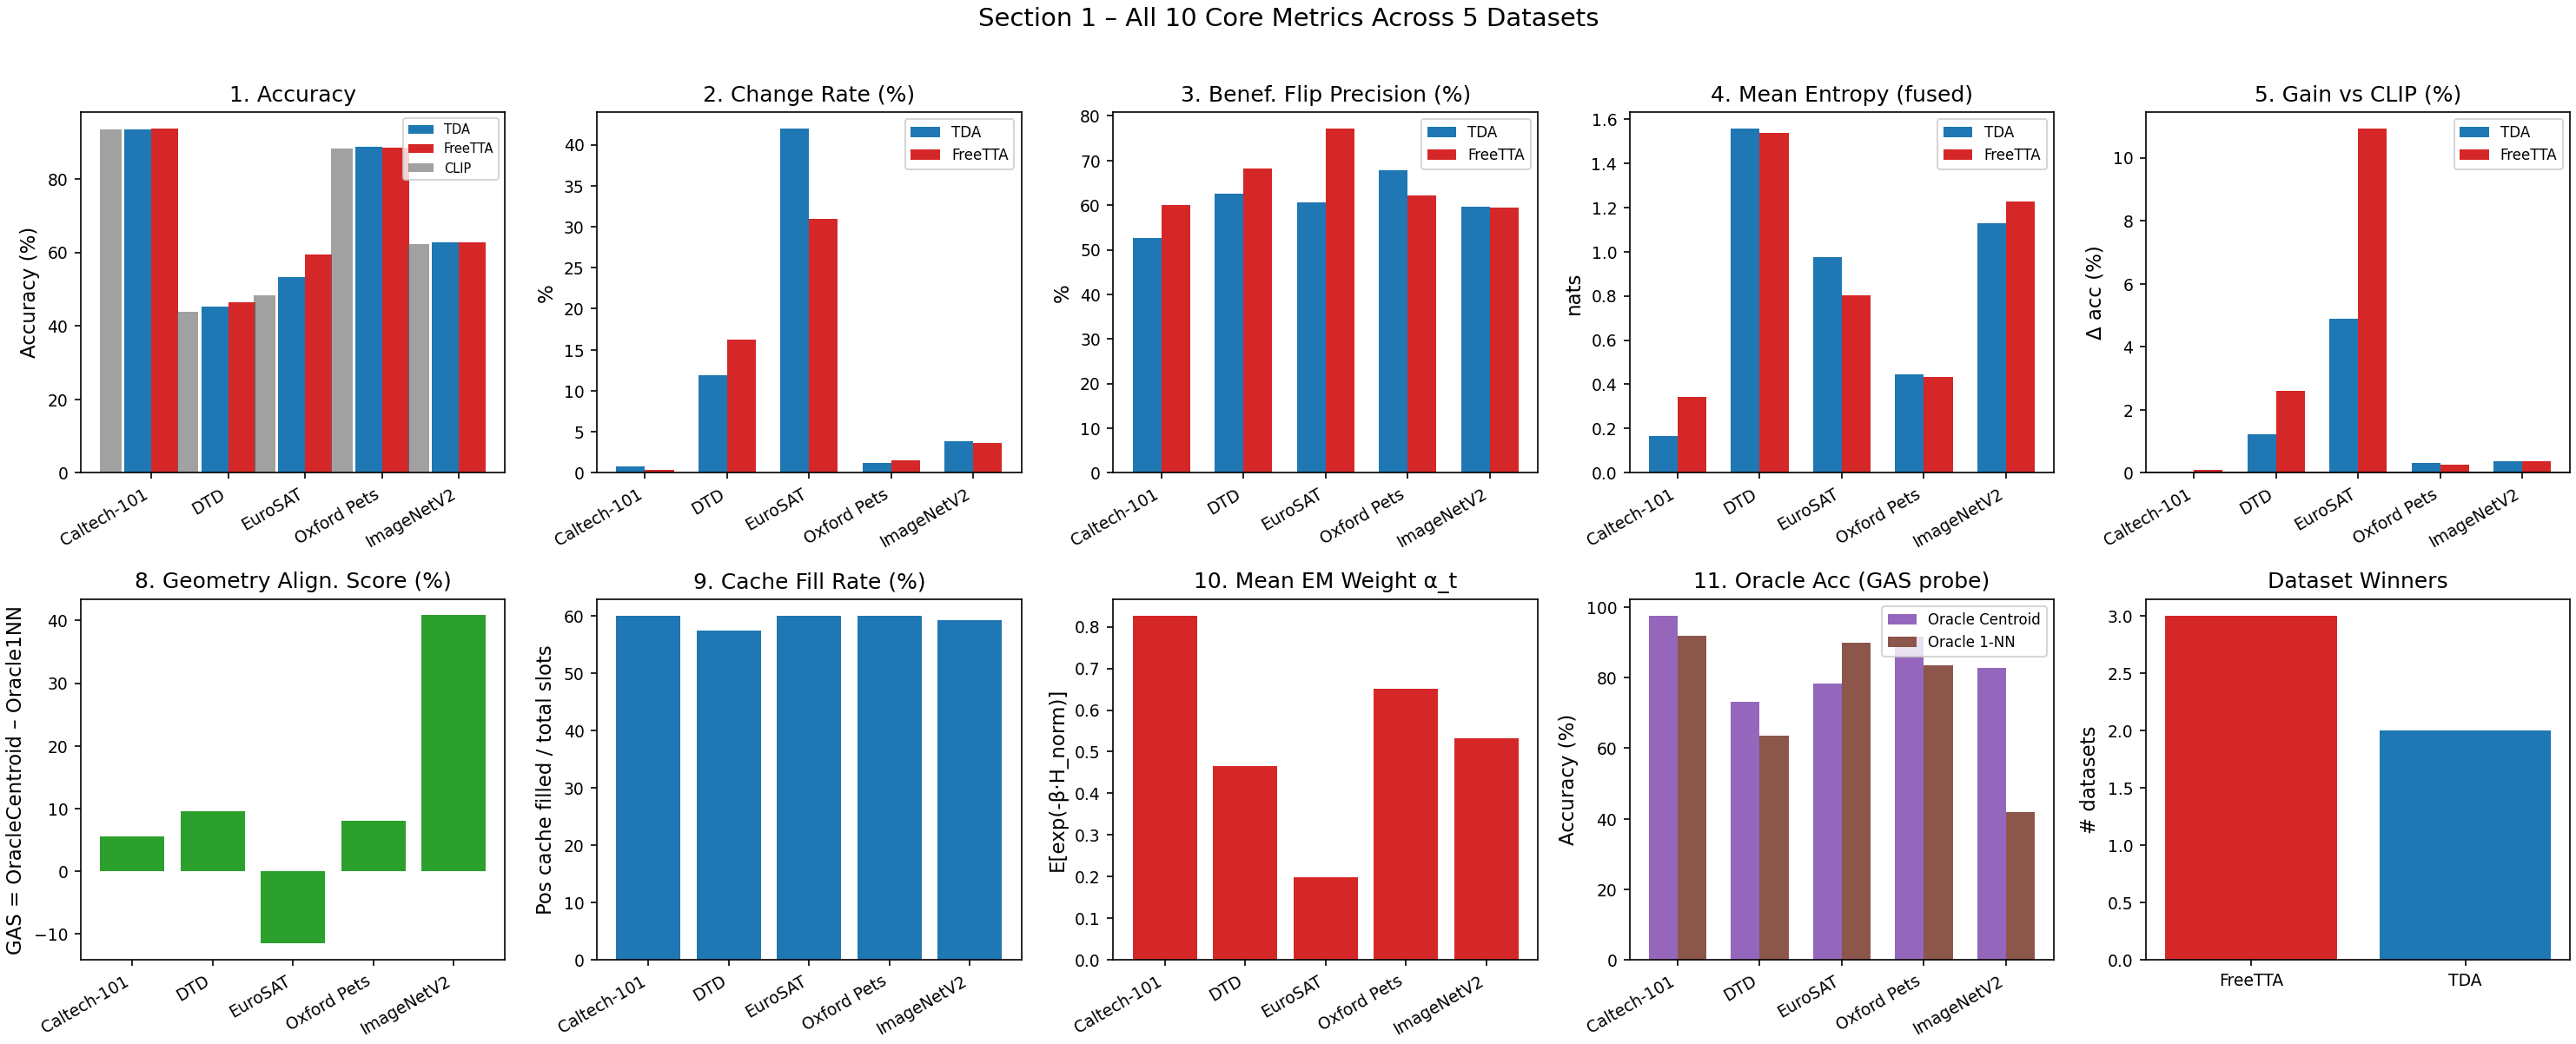
\includegraphics[width=\linewidth,height=0.74\textheight,keepaspectratio]{sec1_all_metrics.png}
\end{columns}
\end{frame}

%% ─────────────────────────────────────────────────────────────────────────────
%% SLIDE 7 – ADAPTATION DYNAMICS
%% ─────────────────────────────────────────────────────────────────────────────
\begin{frame}{Adaptation Dynamics: Rolling Accuracy \& Break-Even}
\begin{columns}[T]
\column{0.60\textwidth}
  \centering
  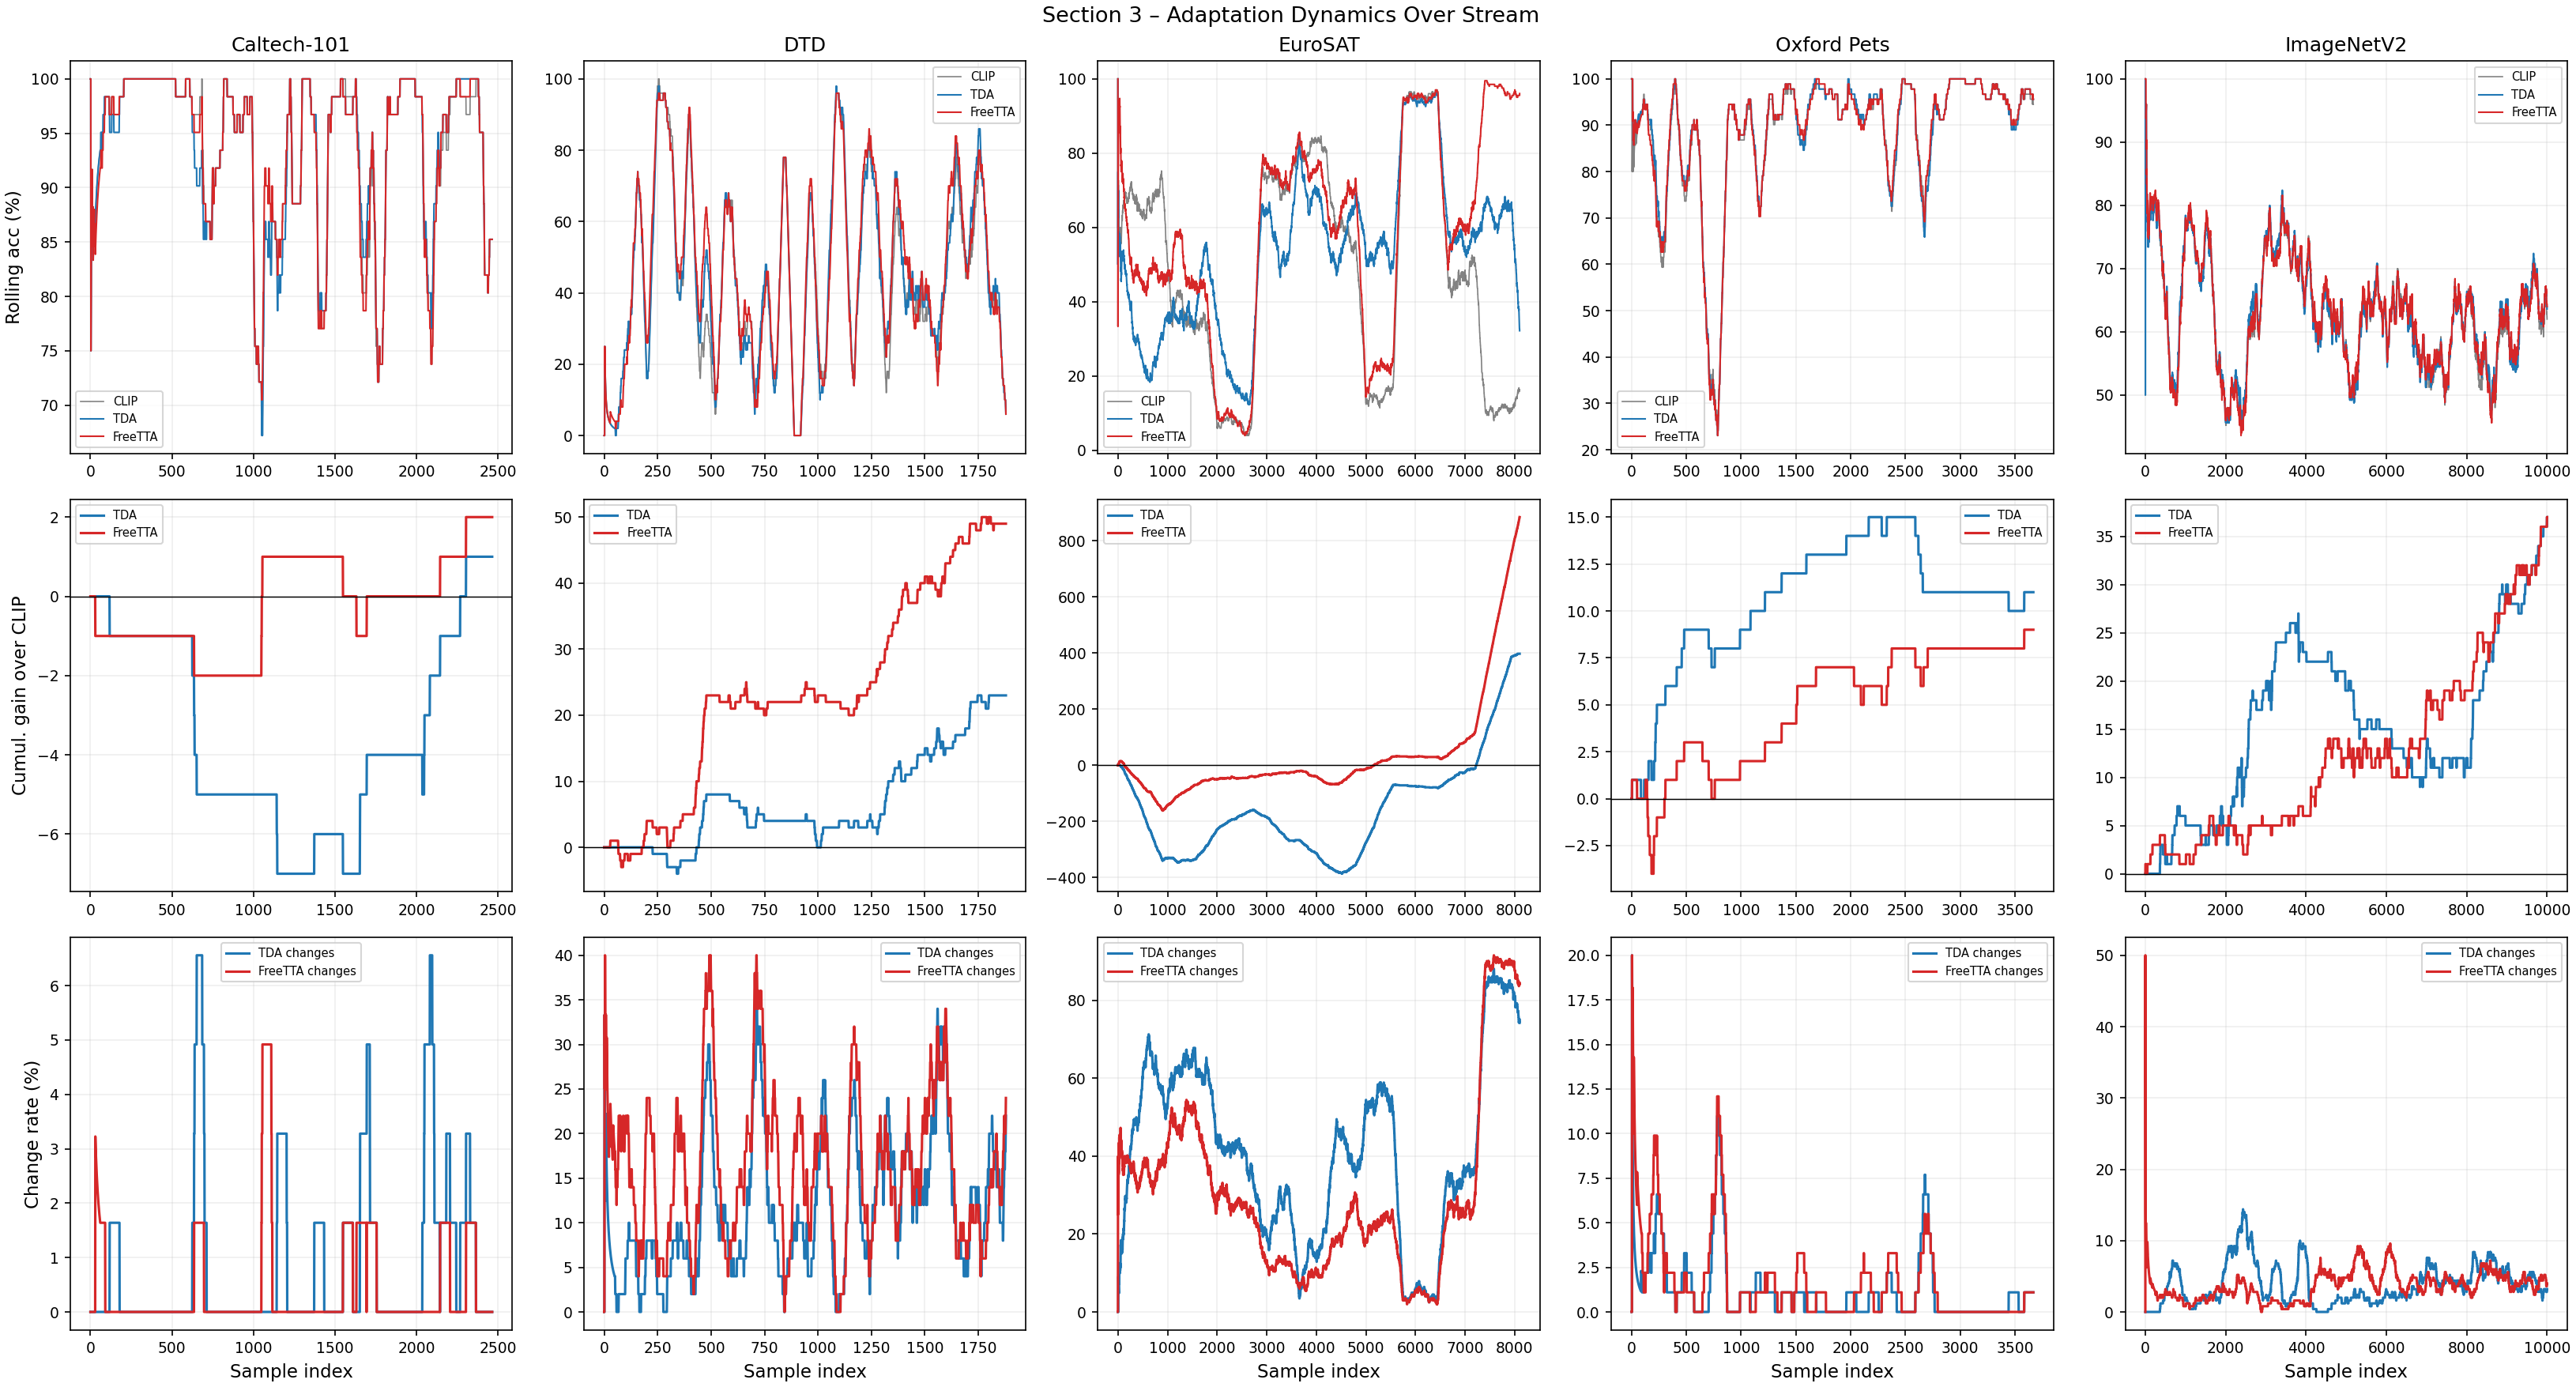
\includegraphics[width=\linewidth,height=0.74\textheight,keepaspectratio]{sec3_adaptation_dynamics.png}
\column{0.38\textwidth}
  \begin{block}{Break-Even Sample}
    \scriptsize When cumulative accuracy first exceeds CLIP:\\[2pt]
    \begin{tabular}{lcc}
      \toprule
      Dataset & TDA & FreeTTA\\
      \midrule
      Caltech  & 2304 & 1055\\
      DTD      & 443  & \textbf{29}\\
      EuroSAT  & 7224 & \textbf{7}\\
      Pets     & 4    & 4\\
      ImageNet & 362  & \textbf{1}\\
      \bottomrule
    \end{tabular}
  \end{block}
  \vspace{3pt}
  \begin{alertblock}{\footnotesize Key Finding}
    \footnotesize TDA on EuroSAT breaks even at sample \textbf{7,224 of 8,100} — helps only the last 11\% of the stream.\\[3pt]
    FreeTTA breaks even at sample \textbf{7}. Adapts 1,000$\times$ faster.
  \end{alertblock}
\end{columns}
\end{frame}

%% ─────────────────────────────────────────────────────────────────────────────
%% SLIDE 8 – SCALING: CONTROLLED EXPERIMENT
%% ─────────────────────────────────────────────────────────────────────────────
\begin{frame}{Scaling: Controlled SPC Experiment (Section 9)}
\begin{columns}[T]
\column{0.60\textwidth}
  \centering
  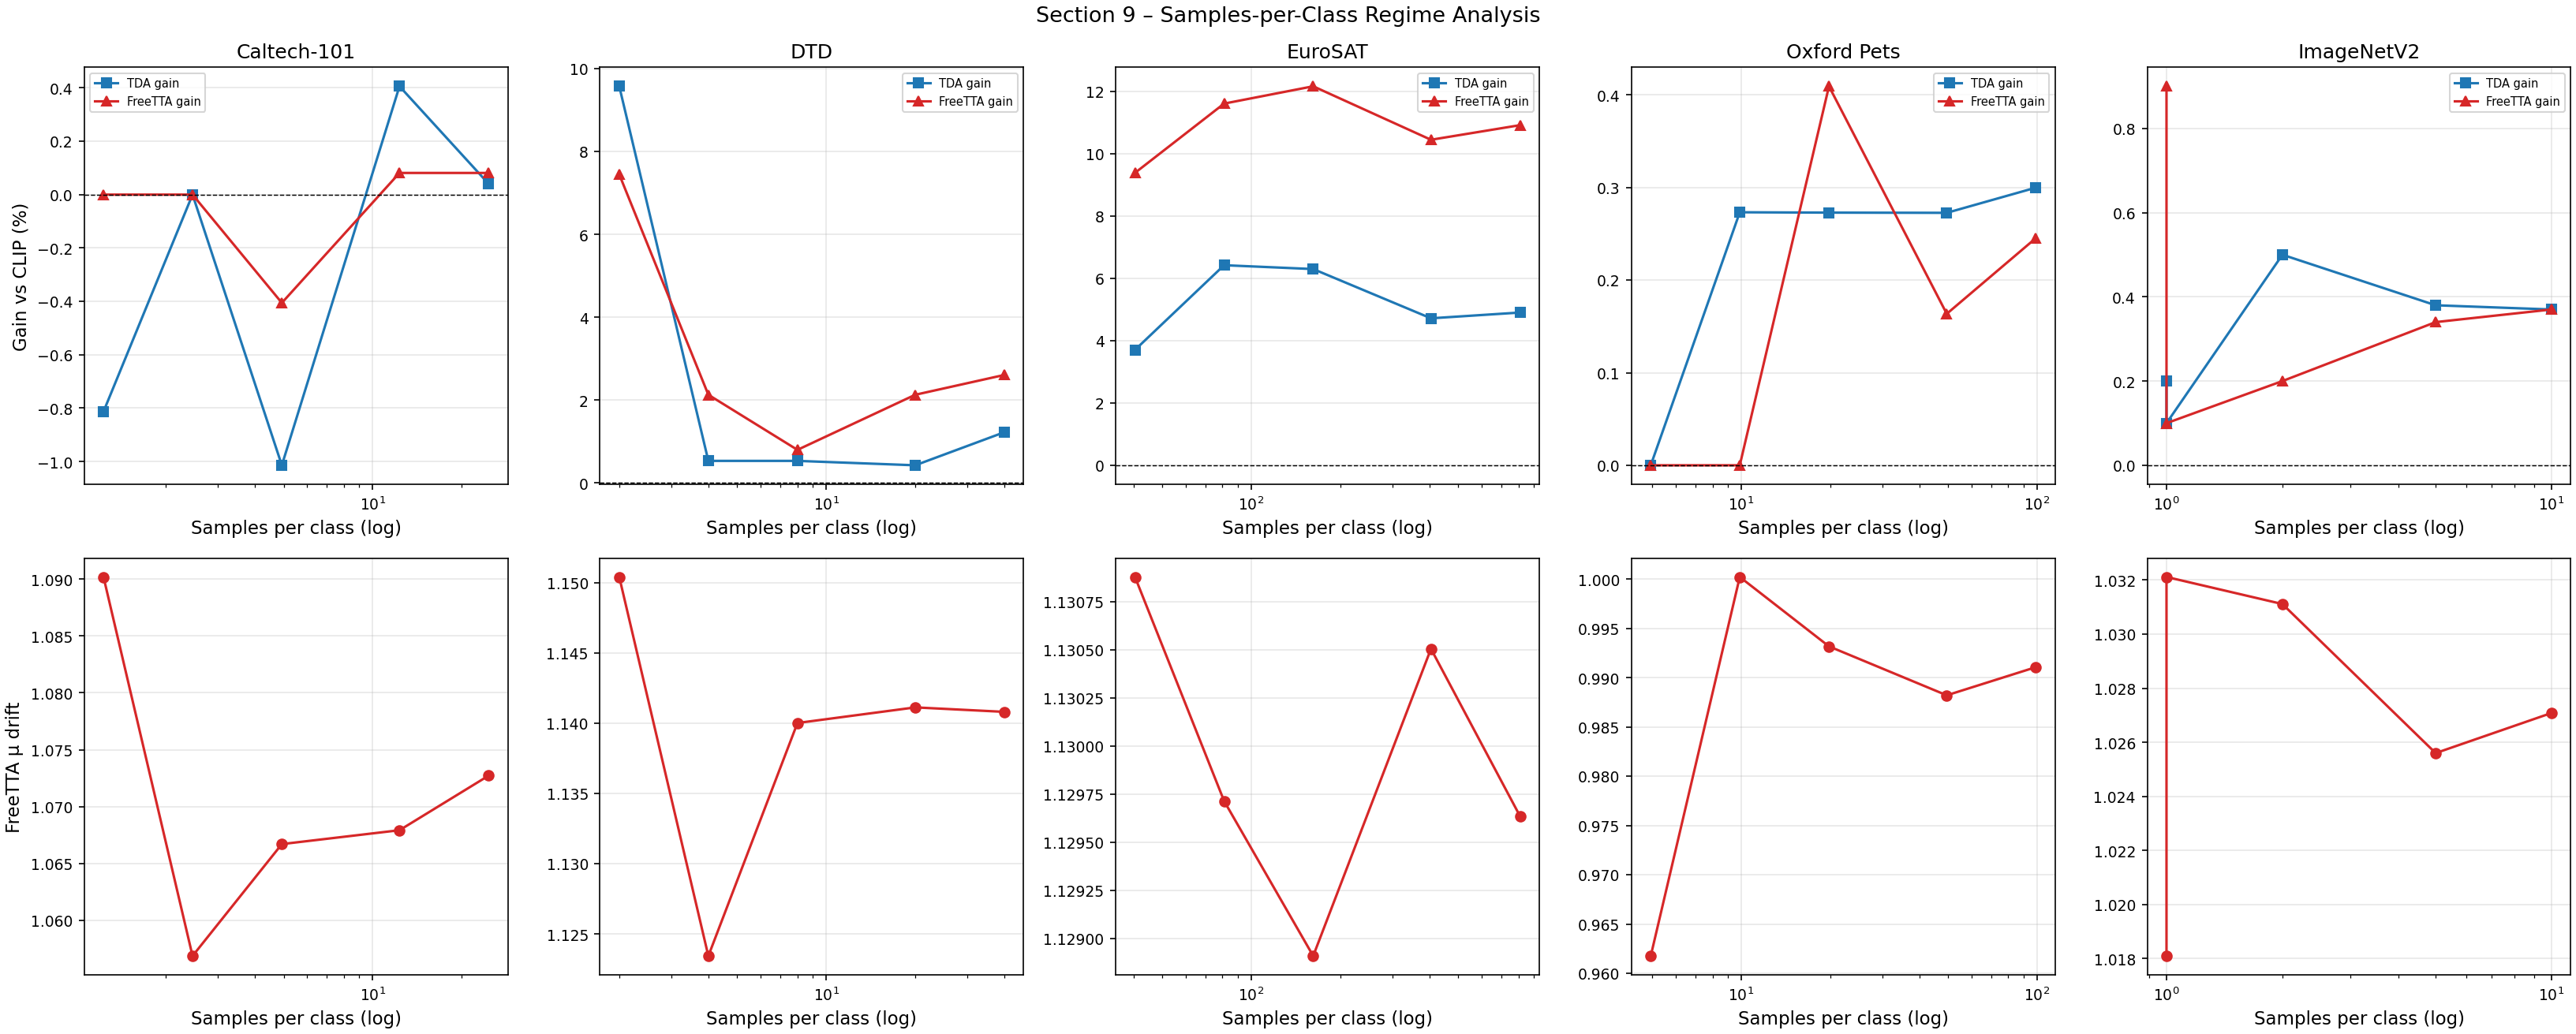
\includegraphics[width=\linewidth,height=0.74\textheight,keepaspectratio]{sec9_spc_regime.png}
\column{0.38\textwidth}
  \begin{block}{EuroSAT Gain vs Stream \%}
    \scriptsize
    \begin{tabular}{lcc}
      \toprule
      Stream & TDA & FreeTTA\\
      \midrule
      5\%  (SPC=40)   & $+2.9$\% & $+5.1$\%\\
      20\% (SPC=162)  & $+3.8$\% & $+8.4$\%\\
      50\% (SPC=405)  & $+4.6$\% & $+9.6$\%\\
      100\% (SPC=810) & $+4.9$\% & $\mathbf{+10.9}$\%\\
      \bottomrule
    \end{tabular}
  \end{block}
  \vspace{3pt}
  \begin{exampleblock}{\footnotesize Interpretation}
    \footnotesize TDA plateaus at $\approx$50\% stream.\\
    FreeTTA gain grows continuously.\\[3pt]
    TDA cache saturates at $C{\times}K{=}30$ exemplars. FreeTTA has no ceiling — each new sample refines $\mub_c$.
  \end{exampleblock}
\end{columns}
\end{frame}

%% ─────────────────────────────────────────────────────────────────────────────
%% SLIDE 9 – UNCERTAINTY ANALYSIS
%% ─────────────────────────────────────────────────────────────────────────────
\begin{frame}{Uncertainty Analysis: Entropy Routing (Section 4)}
\begin{columns}[T]
\column{0.60\textwidth}
  \centering
  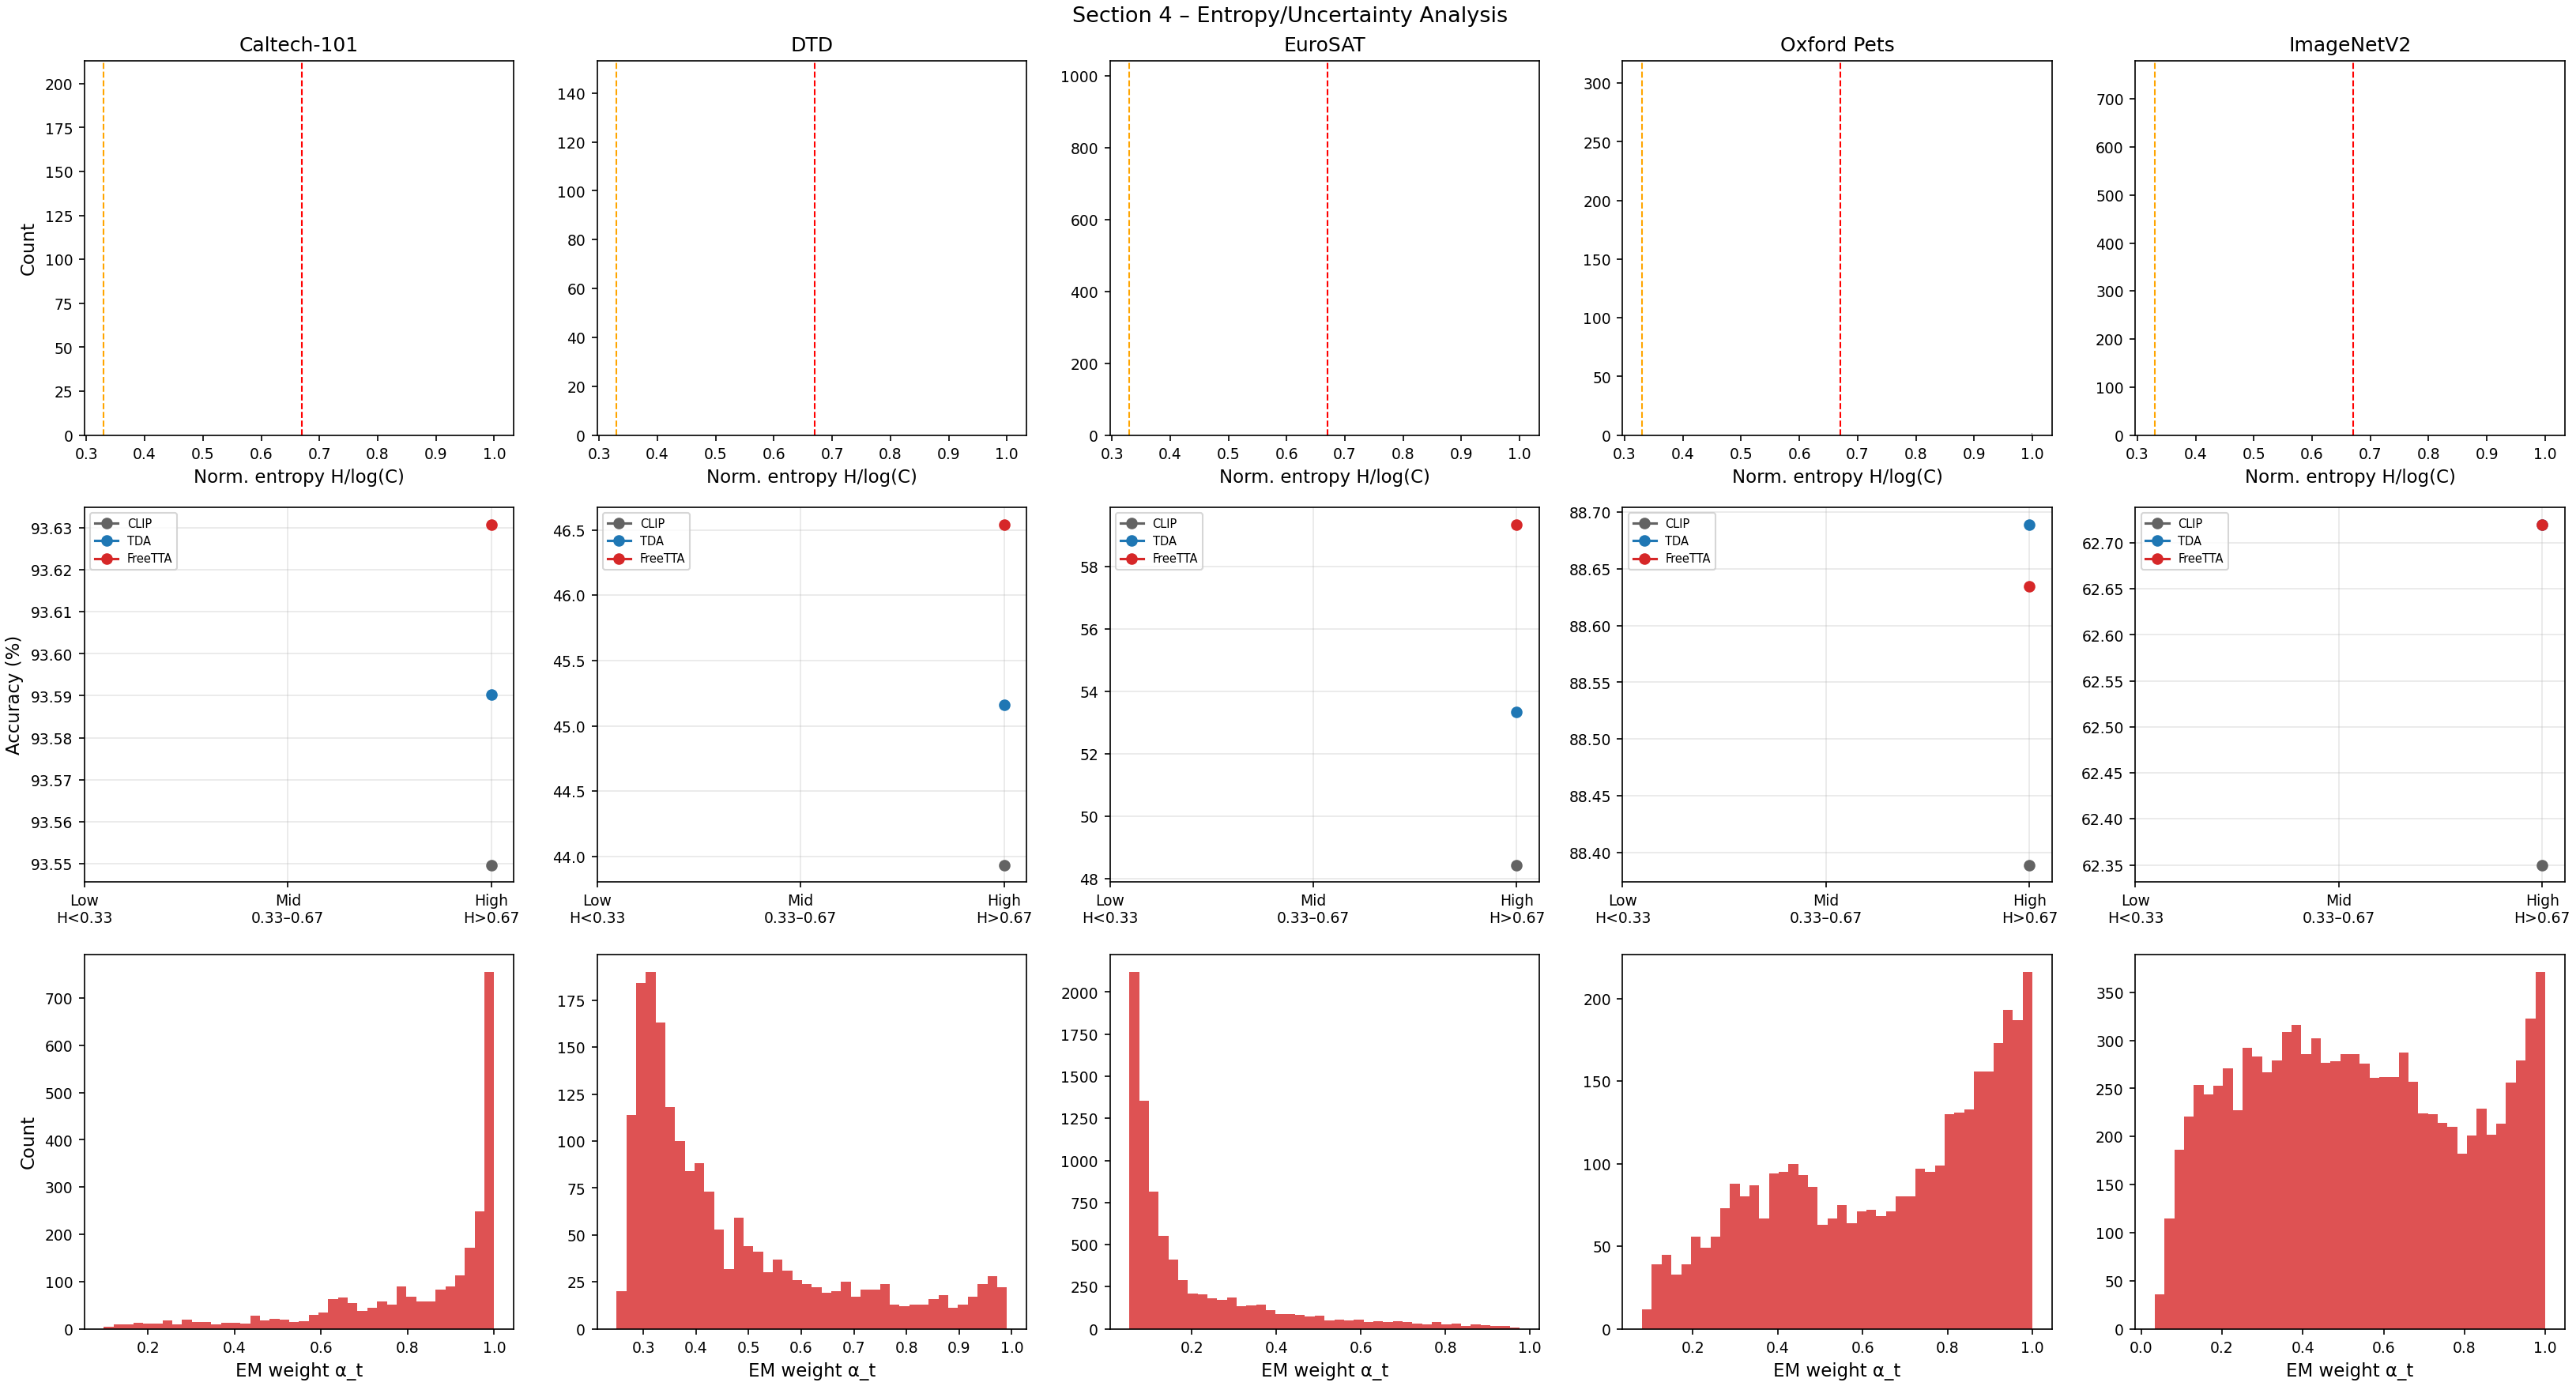
\includegraphics[width=\linewidth,height=0.74\textheight,keepaspectratio]{sec4_uncertainty_analysis.png}
\column{0.38\textwidth}
  \begin{block}{CLIP Entropy Finding}
    \footnotesize CLIP entropy std $= \mathbf{0.000}$ on all 5 datasets.\\[3pt]
    Every sample looks \textbf{identical} to TDA's gate. $H_{\rm norm}\equiv 1.0$ means the gate $[0.2,0.5]$ is \textbf{structurally impossible} — fires 0\% on all benchmarks.
  \end{block}
  \vspace{3pt}
  \begin{block}{\footnotesize EuroSAT Accuracy by Entropy Bucket}
    \scriptsize
    \begin{tabular}{lccc}
      \toprule
      Bucket & CLIP & TDA & FreeTTA\\
      \midrule
      Low H  & 33.6 & 36.6 & \textbf{44.7}\\
      Mid H  & 53.1 & 57.0 & \textbf{63.9}\\
      High H & 58.7 & 66.4 & \textbf{69.4}\\
      \bottomrule
    \end{tabular}
  \end{block}
  \vspace{3pt}
  \begin{alertblock}{\footnotesize Consequence}
    \footnotesize FreeTTA's soft gate $\alpha_t{=}e^{-\beta H}$ is always $>0$. TDA's hard gate: always $0$.
  \end{alertblock}
\end{columns}
\end{frame}

%% ─────────────────────────────────────────────────────────────────────────────
%% SLIDE 10 – CACHE PRESSURE
%% ─────────────────────────────────────────────────────────────────────────────
\begin{frame}{Cache Pressure: Eviction \& Saturation (Section 7)}
\begin{columns}[T]
\column{0.60\textwidth}
  \centering
  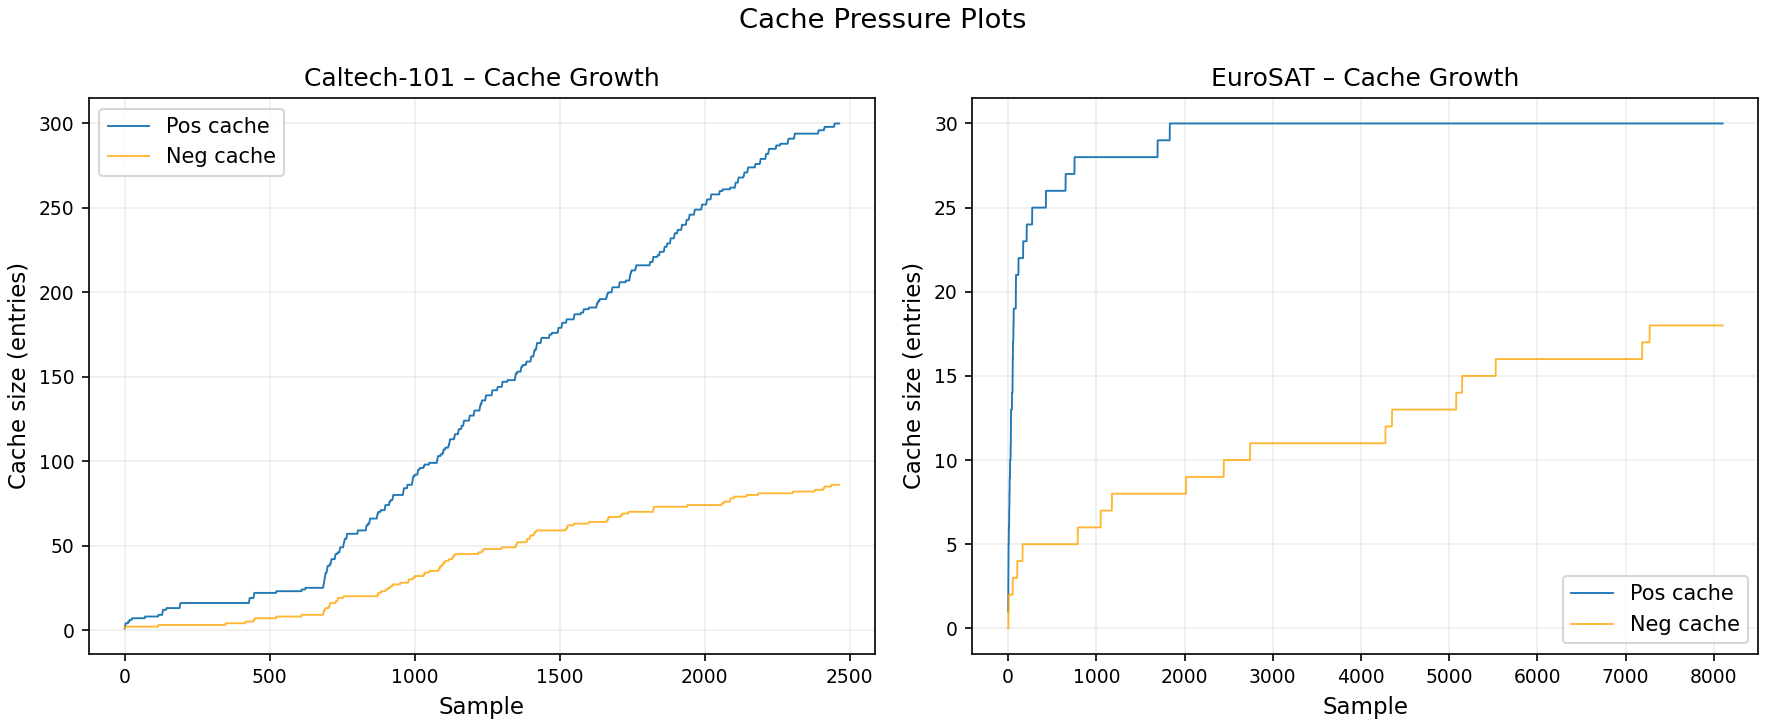
\includegraphics[width=\linewidth,height=0.74\textheight,keepaspectratio]{cache_pressure_plots.png}
\column{0.38\textwidth}
  \begin{block}{Cache Saturation Points}
    \scriptsize Cache fills ($\ge$99\%) after:
    \begin{itemize}\scriptsize\setlength{\itemsep}{1pt}
      \item Caltech: $\sim$300 samples (12\%)
      \item DTD: $\sim$141 samples (7.5\%)
      \item EuroSAT: $\sim$30 samples (0.4\%)
      \item Pets: $\sim$111 samples (3\%)
    \end{itemize}
  \end{block}
  \vspace{3pt}
  \begin{exampleblock}{\footnotesize Eviction Mechanism}
    \footnotesize Per-class slots (cap $K{=}3$). When full: compare incoming entropy to worst slot. Accept only if \textbf{strictly more confident}. After saturation, cache is nearly frozen.
  \end{exampleblock}
  \vspace{3pt}
  \begin{alertblock}{\footnotesize Key Consequence}
    \footnotesize On EuroSAT, TDA's cache is full after just 30 samples. For the remaining 8,070 samples it is essentially a static lookup table, not an adaptive system.
  \end{alertblock}
\end{columns}
\end{frame}

%% ─────────────────────────────────────────────────────────────────────────────
%% SLIDE 11 – DISTRIBUTION MODELING
%% ─────────────────────────────────────────────────────────────────────────────
\begin{frame}{Distribution Modeling: Centroid Drift (Section 5)}
\begin{columns}[T]
\column{0.60\textwidth}
  \centering
  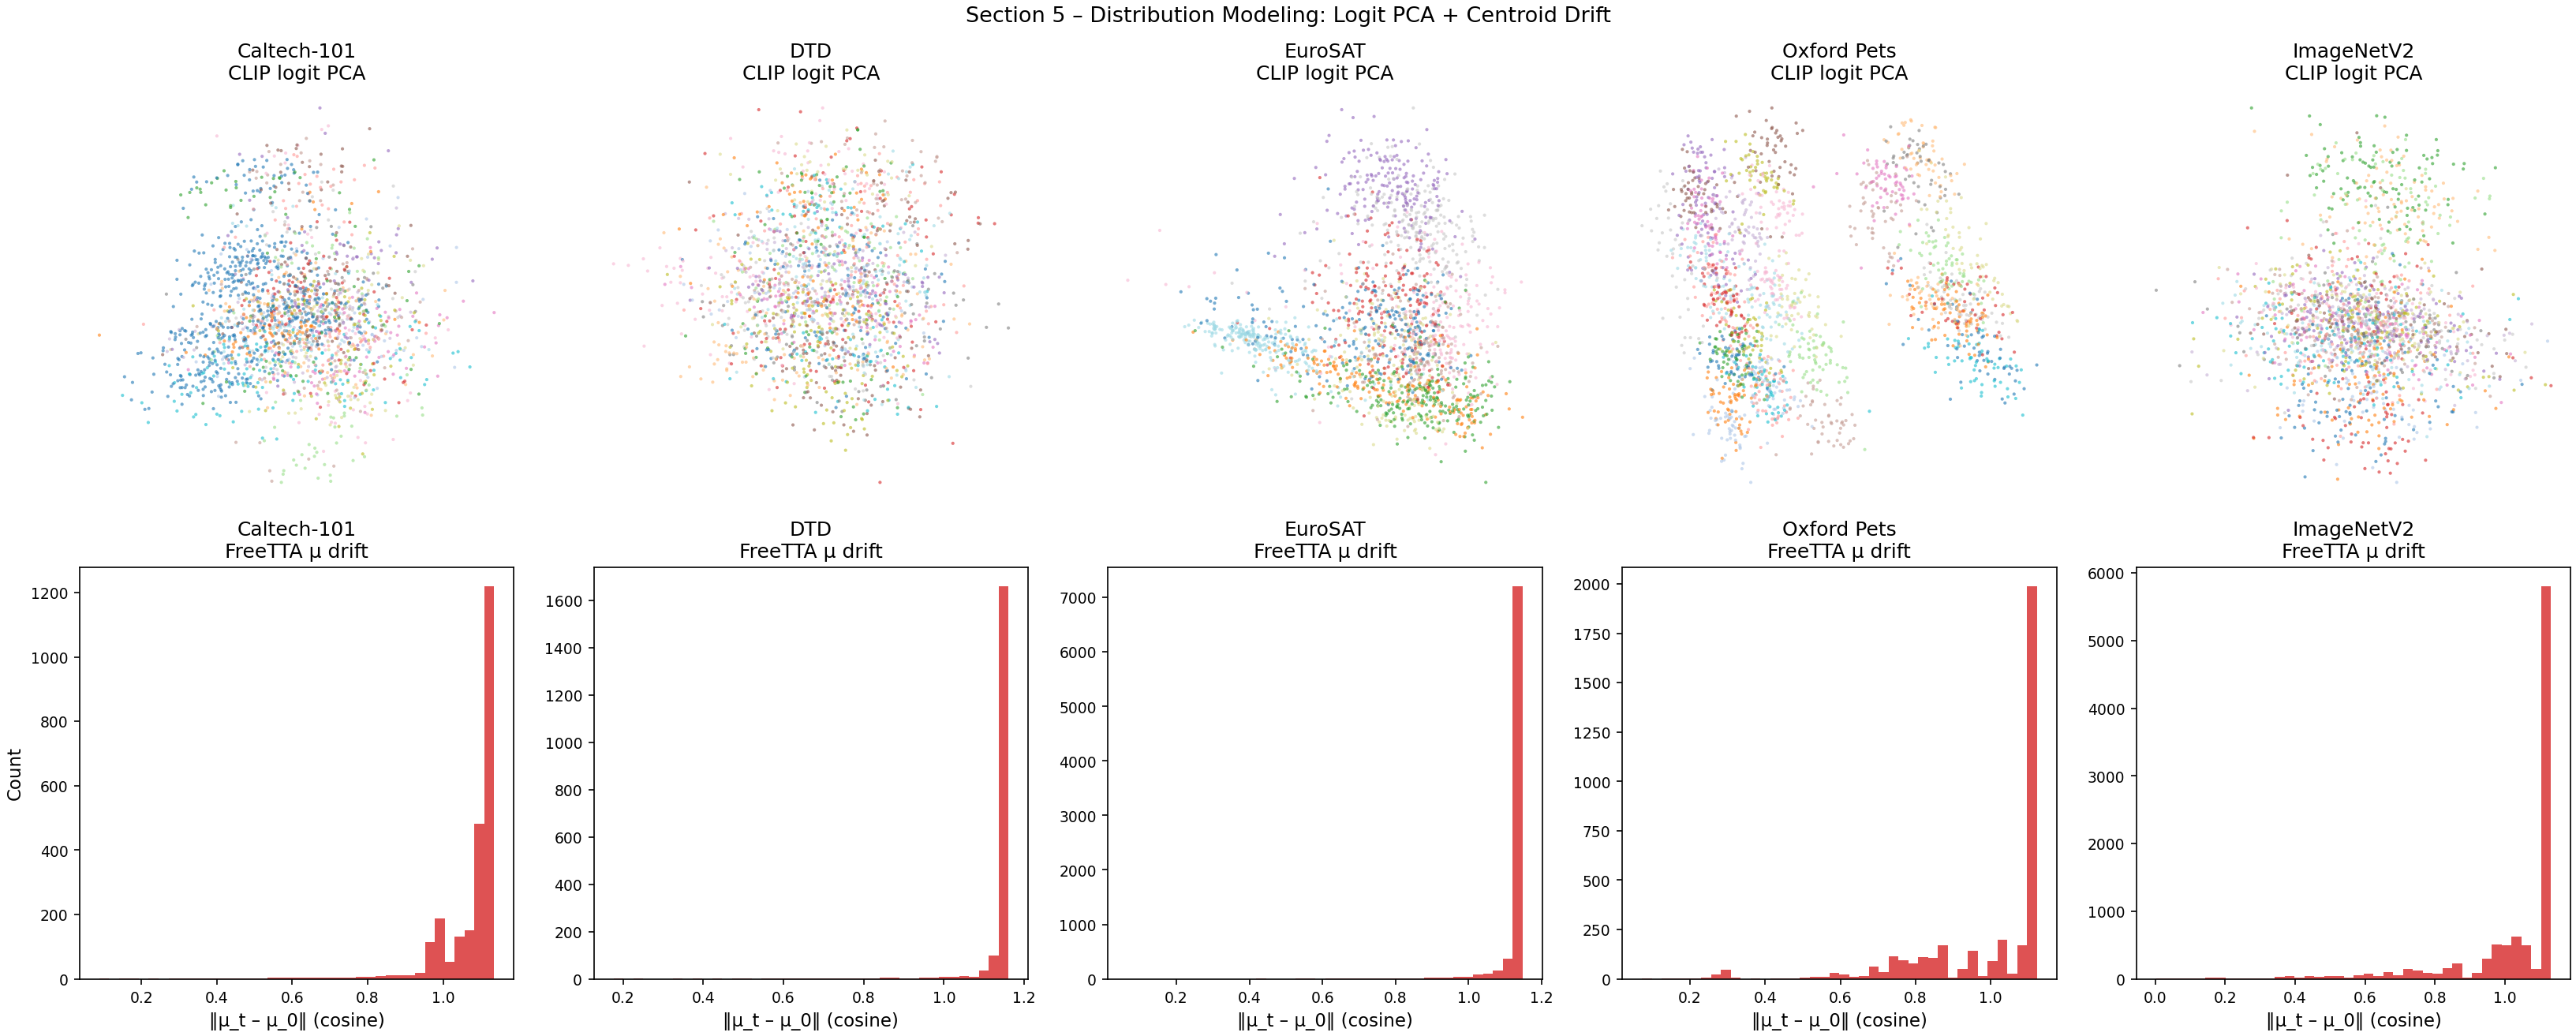
\includegraphics[width=\linewidth,height=0.74\textheight,keepaspectratio]{sec5_distribution_modeling.png}
\column{0.38\textwidth}
  \begin{block}{What FreeTTA Learns}
    \begin{itemize}\footnotesize\setlength{\itemsep}{2pt}
      \item $\mub_c^{(0)} = \hat{\mathbf{t}}_c$ — starts at text embeddings
      \item Each M-step pulls $\mub_c$ toward the image manifold
      \item Drift $\|\mub_c^{(T)}-\mub_c^{(0)}\|$ \textbf{grows throughout} stream
      \item Final $\mub_c^{(T)}$ converges toward true image-space class mean
    \end{itemize}
  \end{block}
  \vspace{3pt}
  \begin{exampleblock}{\footnotesize TDA Has No Analogue}
    \footnotesize TDA cache stores $K{=}3$ exemplars per class — not a distribution estimate. No centroid drift. No convergence property. Cache is a retrieval index, not a distributional model.
  \end{exampleblock}
  \vspace{3pt}
  \begin{alertblock}{\footnotesize Takeaway}
    \footnotesize FreeTTA learns \textbf{where the class lives} in image space. TDA remembers \textbf{a few instances}. On high-shift domains, knowing the class location wins.
  \end{alertblock}
\end{columns}
\end{frame}

%% ─────────────────────────────────────────────────────────────────────────────
%% SLIDE 12 – GAS GEOMETRY ANALYSIS
%% ─────────────────────────────────────────────────────────────────────────────
\begin{frame}{Geometry Alignment Score: Feature Space Structure}
\begin{columns}[T]
\column{0.58\textwidth}
  \centering
  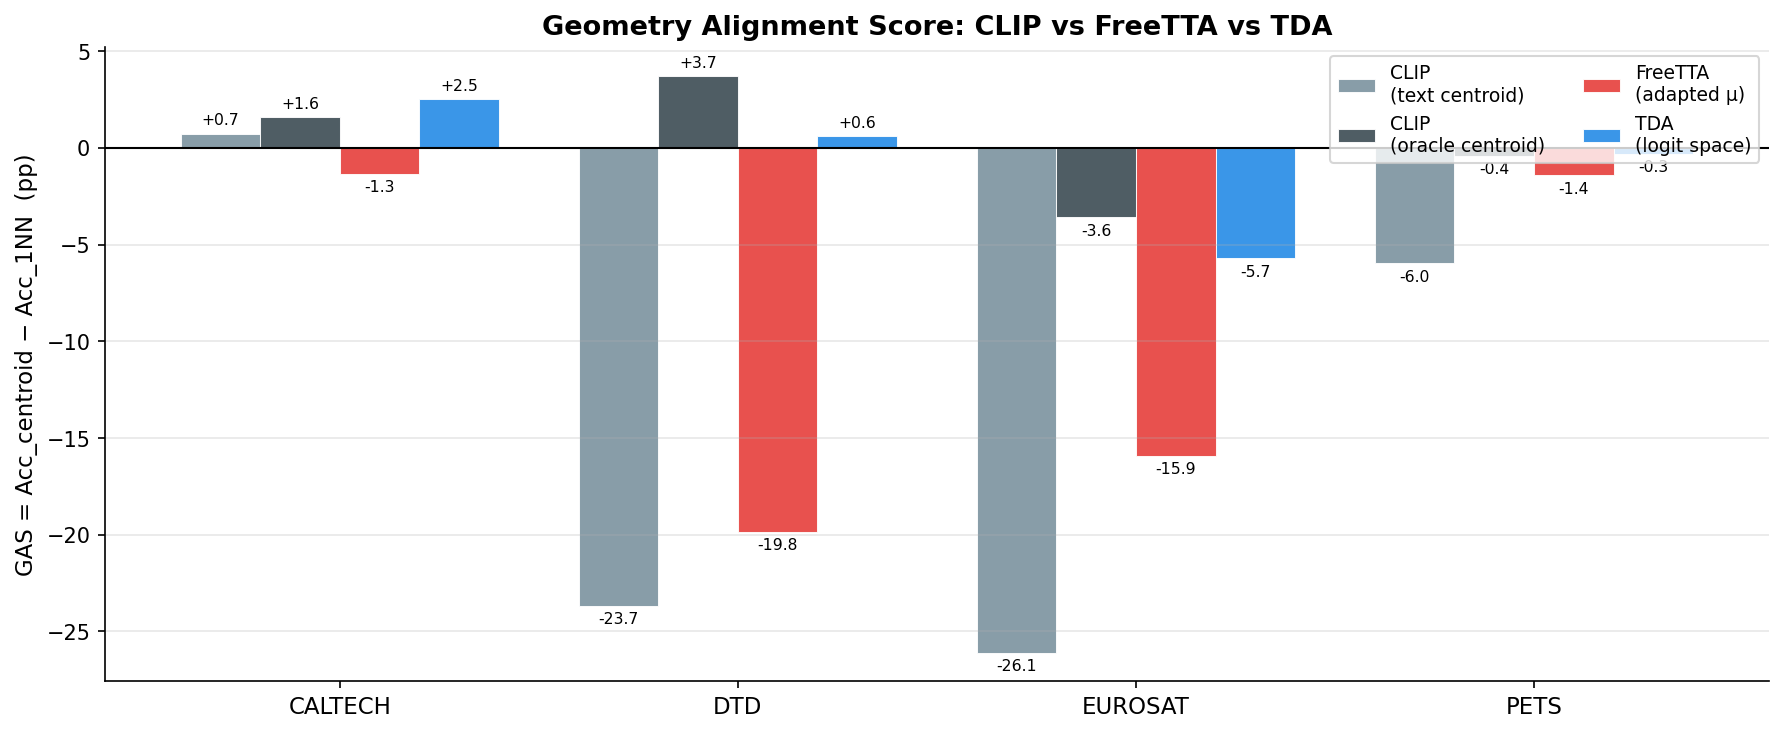
\includegraphics[width=\linewidth,height=0.44\textheight,keepaspectratio]{gas_comparison_bar.png}\\[3pt]
  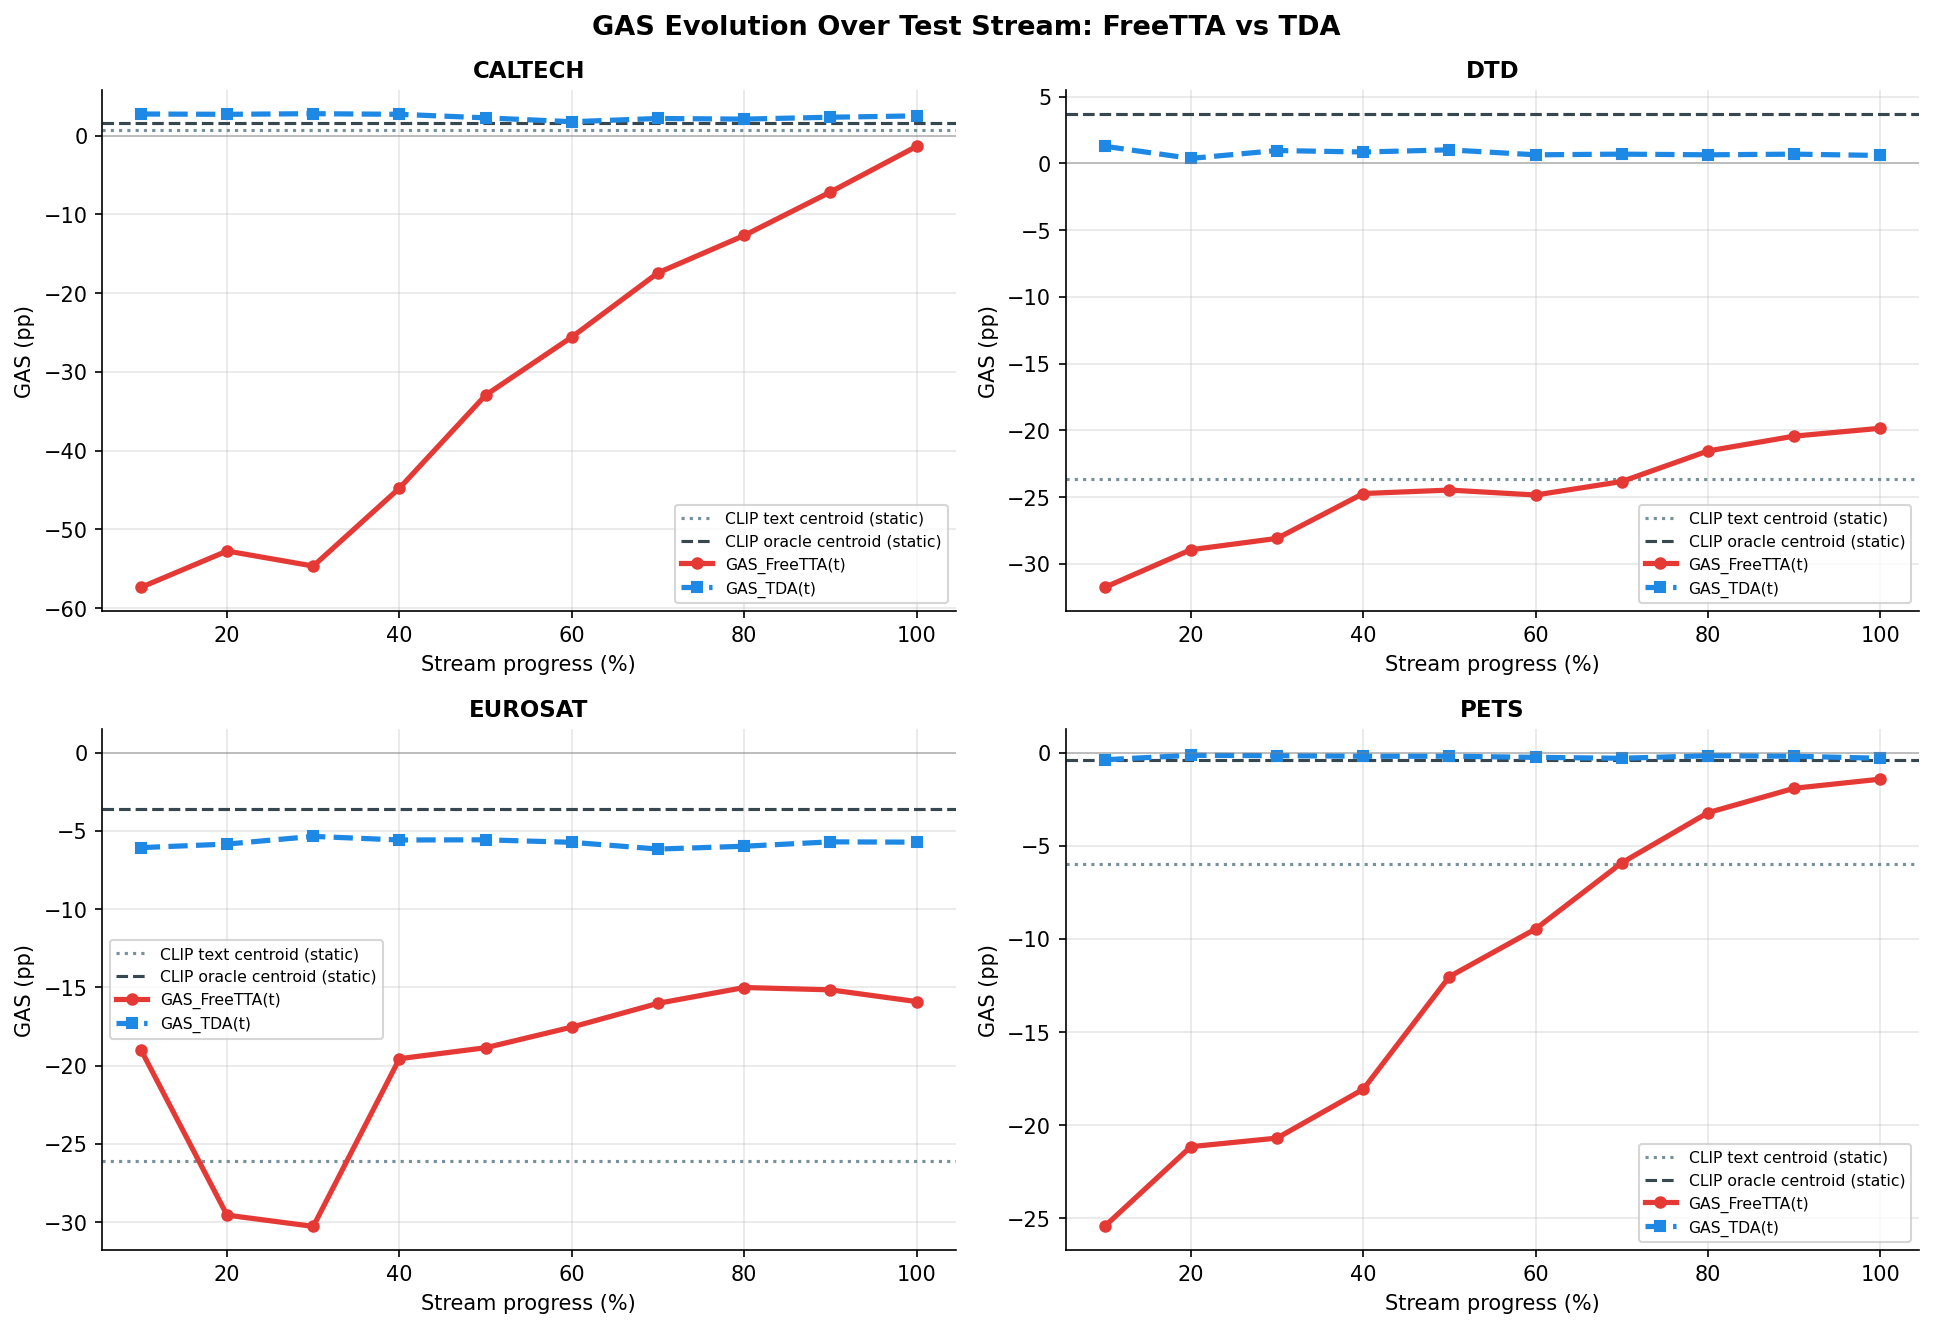
\includegraphics[width=\linewidth,height=0.30\textheight,keepaspectratio]{gas_time_evolution.png}
\column{0.40\textwidth}
  \begin{block}{\footnotesize GAS $=$ Acc$_{\rm centroid} -$ Acc$_{\rm 1-NN}$}
    \scriptsize
    \begin{tabular}{lrr}
      \toprule
      Dataset & FreeTTA & TDA logit\\
      \midrule
      Caltech  & $-1.34$ & $+2.52$\\
      DTD      & $-19.84$ & $+0.59$\\
      EuroSAT  & $-15.91$ & $-5.72$\\
      Pets     & $-1.42$ & $-0.30$\\
      \bottomrule
    \end{tabular}
  \end{block}
  \vspace{3pt}
  \begin{exampleblock}{\footnotesize Interpretation}
    \footnotesize \textbf{TDA} reshapes logit space to be centroid-friendly (GAS improves on all datasets). \textbf{FreeTTA} adapts global class means slowly — GAS starts at $-57$pp and converges over the full stream. \textbf{EuroSAT oracle GAS $=-3.6$}: local structure \emph{inherently} dominates there — explains TDA's relative strength.
  \end{exampleblock}
\end{columns}
\end{frame}

%% ─────────────────────────────────────────────────────────────────────────────
%% SLIDE 13 – ARCHITECTURE COMPARISON
%% ─────────────────────────────────────────────────────────────────────────────
\begin{frame}{Architecture Comparison: Logit Update Mechanisms (Section 15)}
\begin{columns}[T]
\column{0.58\textwidth}
  \centering
  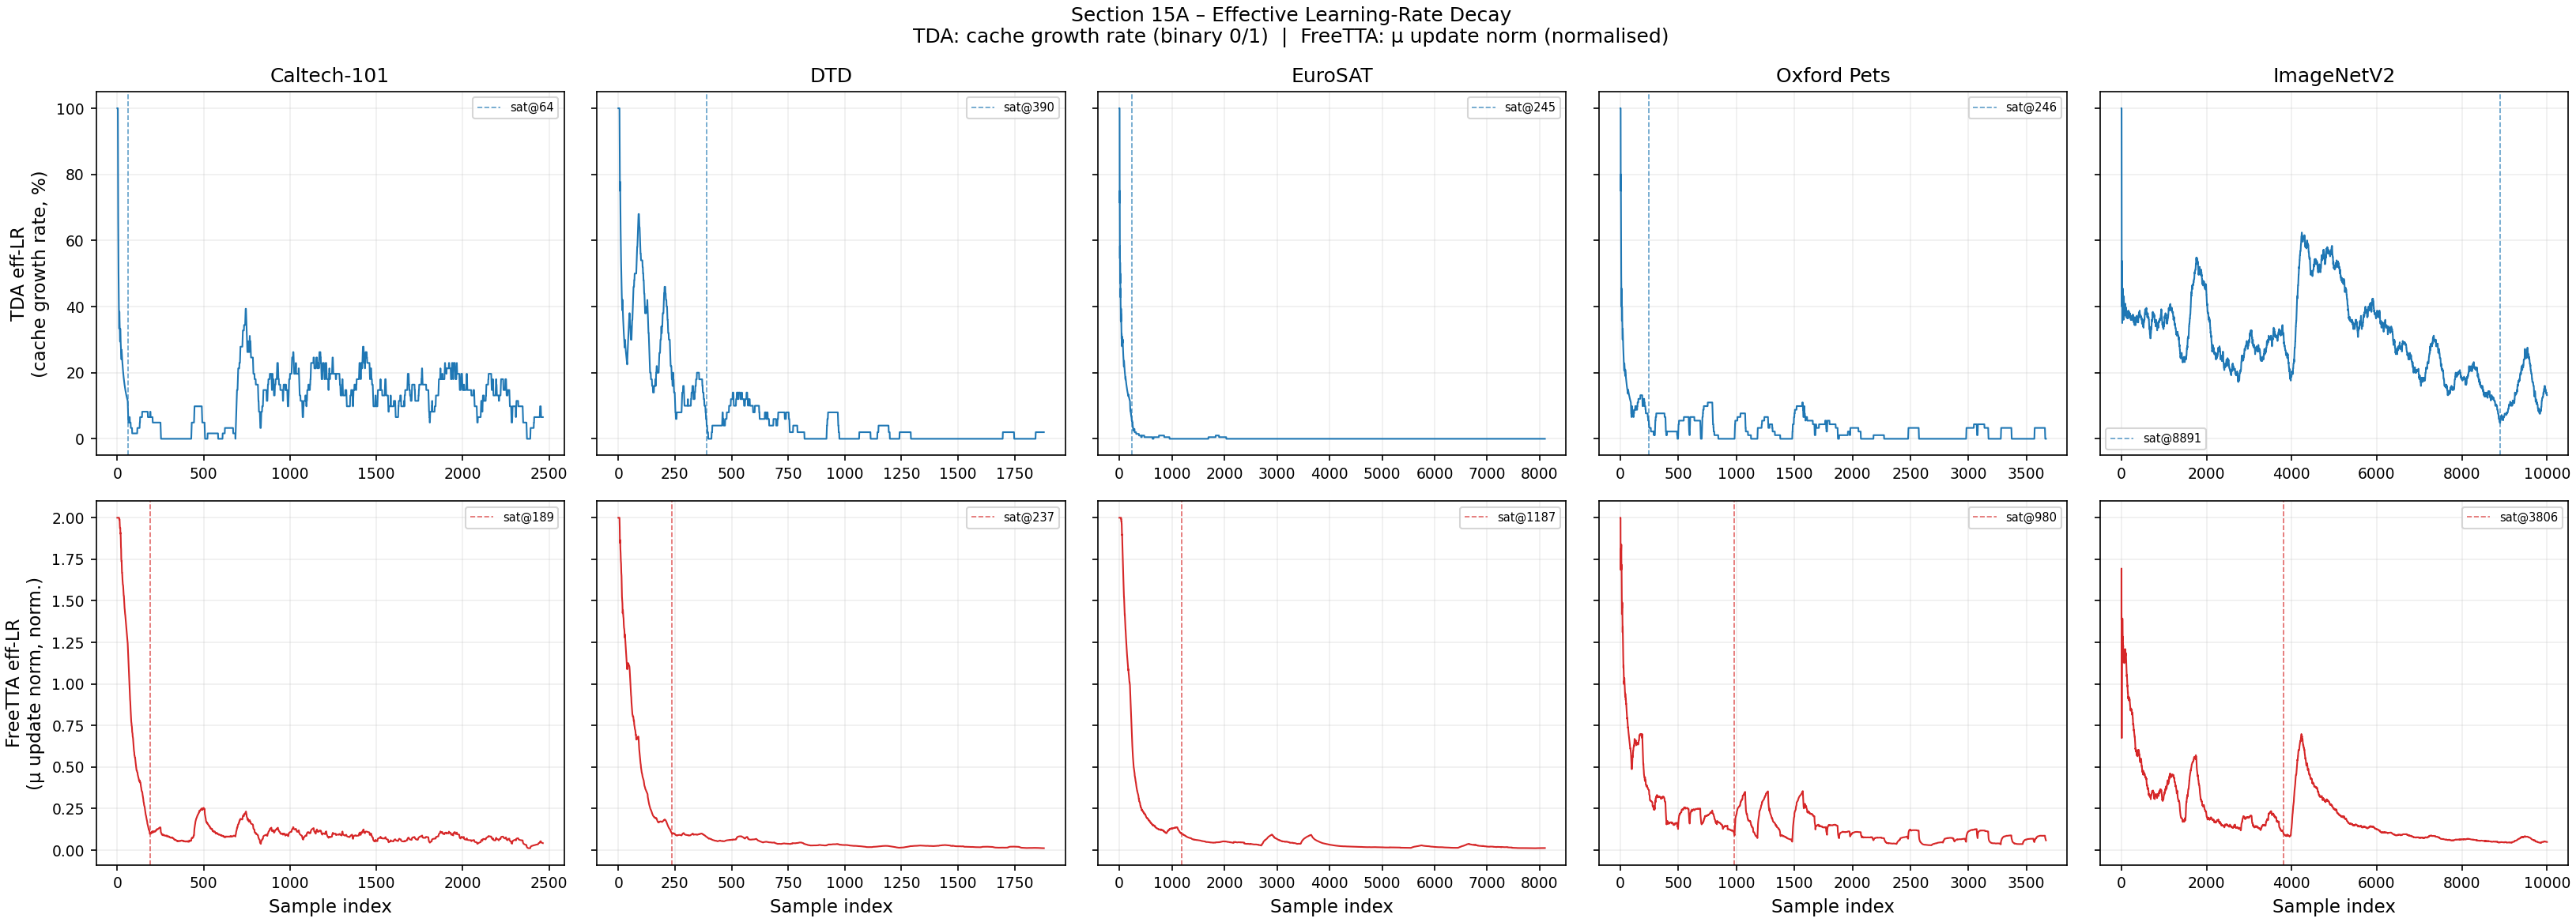
\includegraphics[width=\linewidth,height=0.40\textheight,keepaspectratio]{sec15a_effective_lr.png}\\[4pt]
  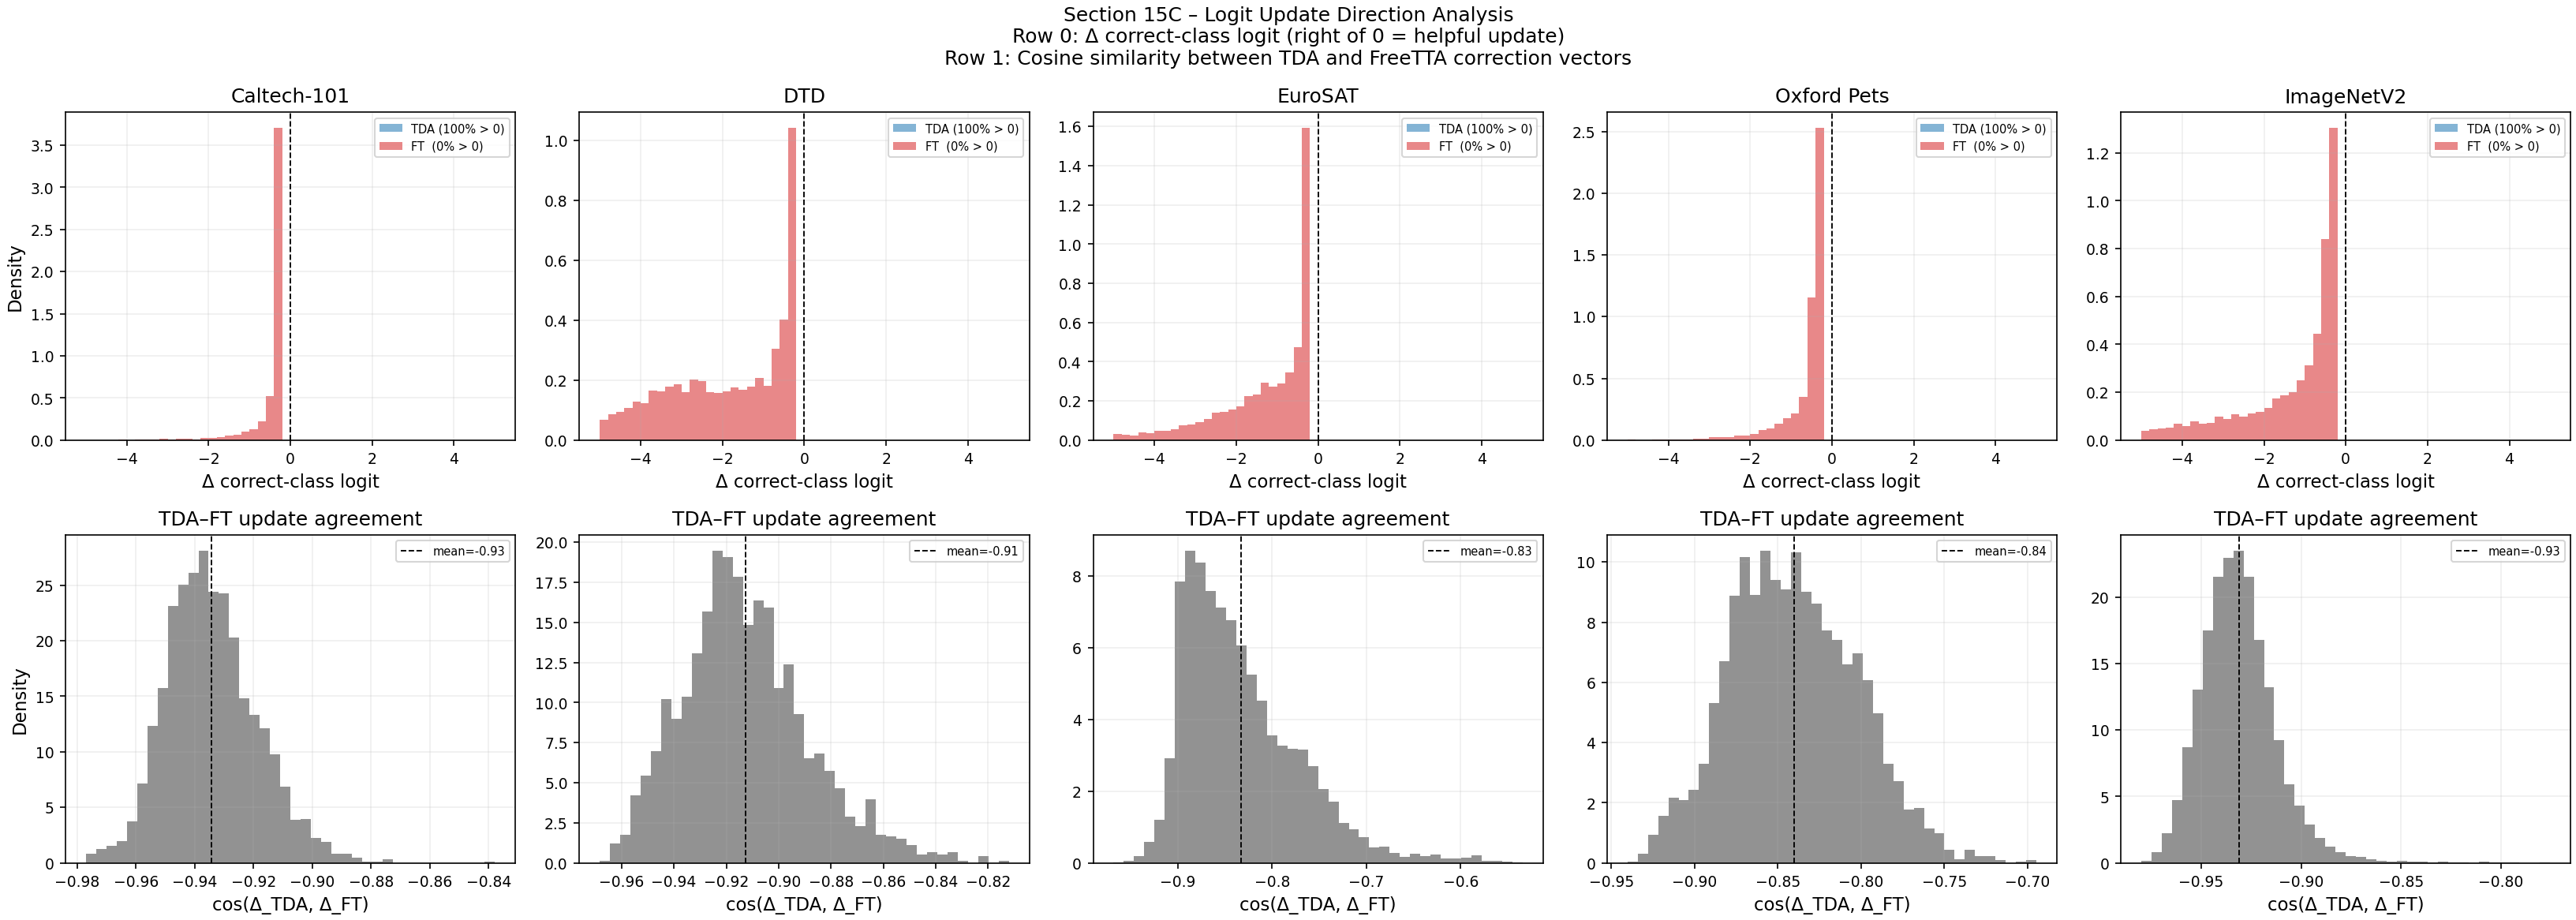
\includegraphics[width=\linewidth,height=0.34\textheight,keepaspectratio]{sec15c_logit_update_direction.png}
\column{0.40\textwidth}
  \begin{block}{\footnotesize Finding 1 — Effective LR Decay}
    \footnotesize \textbf{TDA}: binary $\{0,1\}$ — active only while cache has room; freezes after $C{\times}K$ samples.\\
    \textbf{FreeTTA}: decays as $\sim1/N_y$ — always active, anneals smoothly.
  \end{block}
  \vspace{3pt}
  \begin{alertblock}{\footnotesize Finding 2 — Opposite Directions}
    \footnotesize TDA: $\Delta[y]>0$ for \textbf{100\%} of samples — always boosts correct-class logit absolutely.\\[3pt]
    FreeTTA: $\Delta[y]<0$ for \textbf{100\%} of samples — compresses all logits; wins via relative reranking.\\[3pt]
    $\cos(\Delta_{\rm TDA},\Delta_{\rm FT})\approx\mathbf{-0.9}$ — nearly opposite directions. A logit-level ensemble would cancel out.
  \end{alertblock}
\end{columns}
\end{frame}

%% ─────────────────────────────────────────────────────────────────────────────
%% SLIDE 14 – WHEN EACH METHOD WINS
%% ─────────────────────────────────────────────────────────────────────────────
\begin{frame}{Decision Framework: When Each Method Wins}
\begin{columns}[T]
\column{0.49\textwidth}
  \begin{exampleblock}{FreeTTA Wins When:}
    \begin{itemize}\footnotesize\setlength{\itemsep}{2pt}
      \item \textbf{High domain shift} (EuroSAT): centroids adapt; TDA cache stagnates
      \item \textbf{Long stream} / large SPC: gain grows $+5.1\%{\to}+10.9\%$; TDA plateaus
      \item \textbf{Memory constrained}: 5$\times$ less adaptation memory
      \item \textbf{Fast break-even needed}: starts helping at sample 7 vs 7,224
      \item \textbf{CLIP uniformly uncertain}: soft gate always on vs TDA gate = 0\%
    \end{itemize}
  \end{exampleblock}
\column{0.49\textwidth}
  \begin{alertblock}{TDA Wins When:}
    \begin{itemize}\footnotesize\setlength{\itemsep}{2pt}
      \item \textbf{Low shift + fine-grained} (Pets): cached exemplars match queries closely
      \item \textbf{Short stream}: cache not yet saturated; retrieval precise
      \item \textbf{Local geometry dominant}: oracle GAS $<0$ — 1-NN structure inherent
    \end{itemize}
  \end{alertblock}
  \vspace{4pt}
  \begin{block}{\footnotesize Summary: 5 Key Axes}
    \scriptsize
    \begin{tabular}{lcc}
      \toprule
      Axis & TDA & FreeTTA\\
      \midrule
      Accuracy gain (mean) & $+1.16$\% & $\mathbf{+2.64}$\%\\
      Break-even speed & Slow & \textbf{Fast}\\
      Memory & $5\times$ more & \textbf{Less}\\
      Scalability & Saturates & \textbf{Unbounded}\\
      Gate efficacy & 0\% & \textbf{Always on}\\
      \bottomrule
    \end{tabular}
  \end{block}
\end{columns}
\end{frame}

%% ─────────────────────────────────────────────────────────────────────────────
%% SLIDE 15 – CONCLUSION
%% ─────────────────────────────────────────────────────────────────────────────
\begin{frame}{Conclusion \& Future Work}
\begin{columns}[T]
\column{0.50\textwidth}
  \begin{block}{Key Findings}
    \begin{itemize}\footnotesize\setlength{\itemsep}{2pt}
      \item FreeTTA outperforms TDA on \textbf{3/5} datasets; mean gain $+2.64\%$ vs $+1.16\%$
      \item EuroSAT decisive: FreeTTA break-even sample 7 vs TDA at sample 7,224
      \item TDA neg-cache fires \textbf{0\%}; cache freezes at $<$0.4--12\% of stream
      \item Logit directions: TDA boosts, FreeTTA compresses — cosine $\approx -0.9$
      \item GAS correctly predicts winner in 4/5 cases; fails when domain shift is extreme
      \item Both methods fail on the \textbf{same} 5.8\% of hard samples — CLIP's limit, not adaptation's
    \end{itemize}
  \end{block}
\column{0.48\textwidth}
  \begin{exampleblock}{Future Directions}
    \begin{itemize}\footnotesize\setlength{\itemsep}{2pt}
      \item \textbf{Hybrid}: warm-start FreeTTA $\mub_c$ from TDA cache exemplars
      \item \textbf{Adaptive gate}: adjust $\beta$ dynamically as stream progresses
      \item \textbf{Online GAS routing}: compute GAS from unlabeled stream to select method at inference time
      \item \textbf{Higher-shift benchmarks}: WILDS, medical imaging, satellite time-series
    \end{itemize}
  \end{exampleblock}
  \vspace{4pt}
  \begin{alertblock}{\centering\footnotesize Final Verdict}
    \centering
    \textbf{FreeTTA $\succ$ TDA} for high-shift, long-stream, memory-limited settings.\\[2pt]
    \textbf{TDA} competitive for low-shift, short-stream, fine-grained settings.
  \end{alertblock}
\end{columns}
\vspace{3pt}
\begin{center}
  \scriptsize\textit{36 plots $\cdot$ 22 CSVs $\cdot$ 26,114 samples $\cdot$ 13-section analysis pipeline}
\end{center}
\end{frame}

\end{document}
